\documentclass[12pt,a4paper]{report}
\usepackage[english]{babel}
\usepackage[utf8]{inputenc}

\usepackage[colorlinks]{hyperref}
\usepackage[colorinlistoftodos]{todonotes}

\usepackage[numbers]{natbib}

\usepackage[autostyle]{csquotes}
\usepackage[nottoc]{tocbibind}
\usepackage{indentfirst}

\usepackage[normalem]{ulem}
\usepackage{amsmath}

\usepackage{graphicx}
\graphicspath{ {./images/} }

\newcommand{\defn}[1]{\enquote{\textit{#1}}}
\newcommand{\alleg}{\enquote}
\newcommand{\term}{\textit}
\newcommand{\acronym}{\MakeUppercase}
\newcommand{\itfrac}[2]{\frac{\textit{#1}}{\textit{#2}}}

\begin{document}
	{
		\hypersetup{linkcolor=black}
		\tableofcontents
		\listoftables
		\listoffigures
	}
	
	\chapter{Introduction}
	\label{sec:intro}
	
	During the last years the focus of research for robotic applications evolved 
	from well structured indoor environments to unstructured outdoor environments. 
	With this expansion of interest, it is a crucial prerequisite to reliably 
	classify traversable ground in the environment, especially when it comes to 
	truly autonomous/self-supervised systems. This topic is typically referred to as 
	\term{traversability analysis} or \term{obstacle detection} \citep{Suger}. The 
	verb traverse is defined as \defn{to pass or move over, along, or through}. 
	Hence \term{traversability} refers to the affordance of being able to traverse 
	\citep{Ugur}. Failing on this task can cause great damage or restrict the robots 
	movement unnecessarily.
	\\
	
	So, traversability is the generic capability of a robotic ground 
	vehicle to navigate within environments of varying complexity, while ensuring 
	safety in terms of collisions or reaching unrecoverable states and achieving 
	goals in an optimal mode of operation \citep{Papadakis}. Occasionally other 
	terms such as \term{mobility} \citep{Lalonde}, \term{drivability} \citep{Droeschel}, 
	etc are used to describe the same concept.
	\\
	
	Although traversability is considered a fundamental capability for mobile 
	robots, in some cases it is limited to the problem of simple obstacle avoidance 
	\citep{Ugur}. When such approaches are used, the robot tries to avoid making any 
	physical contact with the environment, and heads only to open spaces. Its 
	response would be the same whether it encounters an impenetrable wall or a 
	balloon that can just be pushed aside without any damage. Therefore, methods 
	that can automatically learn the traversability affordances from the 
	robot’s interactions with the environment are valuable for robotics.
	\\
		
	In addition, there is the possibility that previously learned behavior is not 
	relevant, because the visual appearance and traversability of roads may 
	have changed due to various reasons \citep{Wigness}. That is probably why 
	geometry-based analysis is the direction followed by the majority of 
	traversability analysis methodologies in the past \citep{Papadakis}.
	\\
	
	Supervised learning approaches are unlikely to work reliably in unknown or 
	unstructured outdoor environments. That is because the system assesses the 
	traversability using an off-line learned model trained with specific 
	terrain types. For example, if a system is trained with terrain samples in a 
	specific season, the systems might not detect traversable regions in other 
	seasons \citep{Lee}.
	\par
	Unsupervised, or else self-supervised, learning approaches may be the solution 
	to this problem. They use on-line learning methods in order to exploit newly-
	acquired training data in making traversability predictions about unknown 
	terrain \citep{Kim}. That way the learned traversability concepts are 
	incrementally updated with new data only. That comes with the advantage that the 
	updated classifier is immediately available for navigation and that the memory 
	requirements for learning are reduced, compared to off-line methods.
	\par
	In the real world and its unstructured and dynamic surroundings such as vegetation 
	landscape and terrain, the perception of a mobile robot needs to be capable of 
	navigating this unknown environment by using sensor modalities \citep{Shabbir}.
	\\
	
	So, if autonomous mobile robots are to become more generally useful, they must 
	be able to adapt to new environments and learn from experience. To do so, they 
	need a way to store pertinent information about the environment, recall the 
	information at appropriate times, and reliably match stored information with 
	newly-sensed data. They also must be able to modify the stored information to 
	account for systematic changes in the environment \citep{Shneier}.
	\\
	
	Estimating the traversability of terrain in an unstructured outdoor 
	environment is a core functionality for autonomous robot navigation \citep{Kim}. 
	Nevertheless, the traversability of more complex terrain, such as 
	vegetation and sloping ground, is extremely difficult to characterize beforehand. 
	It is difficult to find general rules which work for each vehicle's	capabilities
	and for a wide variety of terrain types such as trees, rocks, tall grass, logs, 
	and bushes. As a result, methods which provide traversability estimates 
	based on predefined terrain properties such as height, shape or colour 
	(\term{geometry-based} and \term{appearance-based} analyses) will be unlikely to 
	work reliably in unknown outdoor environments. That is why combining data 
	collected a priori together with the vehicle’s navigation experience is more 
	likely to work better for deciding terrain traversability (see more about 
	\term{hybrid} approaches in \citet{Papadakis}).
	\\
	
	Last but not least, traversability should be treated as an affordance and 
	not simply as a predefined property of different types of terrain \citep{Kim}. 
	That is because a large vehicle may be able to drive over small saplings that 
	would present an insurmountable obstacle to a smaller vehicle. A stair that is 
	traversable for a hexapod robot may not be traversable for a wheeled one. So, 
	when used here, \term{affordance} implies the complementarity of the robot and 
	the environment, the interaction between them \citep{Ugur}.
	\\
	
	In this thesis we will tackle on how an autonomous mobile robot can improve its 
	traversability estimation method in natural environments, meaning not 
	only on bare ground-like environment but also on terrain containing vegetation. 
	On contrast, we will rule out high-risk applications where a single accident can 
	be fatal to the robot like planetary or volcano exploration. We will concentrate 
	in everyday practical situations. We will determine how to introduce a learning 
	capability to the robot that will enable it to decide for itself the 
	traversability of the terrain around it, based on input from its sensors 
	and its experience of traveling over similar terrain in the past. We would also 
	like our robot to plan further ahead and avoid entering traps that prevent it 
	from reaching its goal.
	\\\\
	
	The rest of the thesis is organized as follows:
	\begin{itemize}
		\item In Chapter~\ref{sec:bg} we give a background on the topic we are dealing 
		with. We present already existing traversability estimation algorithms; the 
		goals, the approaches, the methods used, the strengths and weaknesses. 
		\item In Chapter~\ref{sec:fg} we present the logic behind the decisions made 
		and the algorithms used.
		\item In Chapter~\ref{sec:exp} we perform an evaluation of our implementation 
		and compare it with previous ones.
		\item In Chapter~\ref{sec:concl} we give our conclusions and ideas for future 
		work.
		\item In Appendix~\ref{app:impl} we share some \acronym{url}s of prototype 
		implementations from researchers who kindly offered their work open-source.
		\item In Appendix~\ref{app:conv} one can find a brief outline on how 
		convolutional neural networks work.
	\end{itemize}
	
	\chapter{Background}
	\label{sec:bg}
	
	\section{A few words}
	\label{sec:bg:intro}
	
	In order to have an autonomous robot improve its traversability 
	estimation we will need to address each sub-problem individually:
	
	\begin{enumerate}
		\item Traversability estimation algorithms that can be improved from 
		experience/examples.
		\item Methods for collecting the data needed by the algorithm above, from 
		the sensory input that is available to the robot. (The input we have does not 
		directly map to positive/negative decision).
		\item Navigation strategies. There might be an explicit goal to achieve, e.g.
		follow the fastest or easiest route to a target. Or it could be curiosity-driven 
		exploration, meaning the abstract need to learn a new environment.
	\end{enumerate}
	
	We will now present the state of the art in all three areas of research.
	\\
	
	\section{Learning traversability estimation algorithms}
	\label{sec:bg:trav}
	
	In order for an autonomous robot to be able to safely navigate, it is crucial 
	for it to be able to conclude on its own the terrain traversability 
	around it. Historically, most commonly, traversability analysis is 
	treated as a binary classification problem \citep{Papadakis}, i.e. distinguishing 
	traversable from non-traversable terrain. But later on, it became clear that 
	rough natural terrain is not easily partitioned into clear traversable and non-
	traversable classes. The need for finer classification was recognized. The new 
	idea was to either assign a continuous traversability score or classify 
	the terrain into the various classes that were commonly encountered within a 
	particular application. Many papers have been published regarding 
	traversability estimation approaches, and here we present some of the 
	most recent and most influential.
	\\
	
	This line of research starts with \citet{Lalonde} that segment local three-
	dimensional (\acronym{3d}) \term{point clouds} using a purely geometric 
	approach, for autonomous robot navigation purposes. A 
	\term{point cloud} is a set of data points in space, generally produced by 
	\acronym{3d} scanners. The approach used is a segmentation in three terrain 
	categories, based on scatter-ness, linear-ness, and surface-ness. That way 
	the authors are able to represent porous volumes such as grass and tree canopy, 
	capture thin objects like wires or tree branches, and capture solid objects 
	like ground surface, rocks or large trunks, respectively.
	\\	
	
	A different line of research starts with \citet{Pfaff} that decided to represent 
	the environment of a mobile robot with \term{elevation maps}, another geometric 
	approach. A \term{digital elevation map (\acronym{dem})} \citep{Kweon} is also 
	known as a \term{2\(\itfrac{1}{2}\)-dimensional representation} of the environment 
	\citep{Pfaff}. It is a two-dimensional (\acronym{2d}) array of terrain elevation 
	measurements. More concrete, it is a grid that stores in each cell the vertical 
	distance above or below the corresponding surface, the height of the territory. 
	\par 
	The representation of the environment with elevation maps, however, can 
	be problematic when a robot has to utilize these maps for navigation. For 
	example, when a mobile robot is located in front of a bridge, the underpass will 
	completely disappeared and the elevation map will show a non-traversable 
	object.
	\par
	\todo[size={{\scriptsize}}]{Explanation of representation and traversability of the area under the bridge}
	\citet{Pfaff} classify the cells of elevation maps into four classes: 
	parts of terrain seen from above, vertical structures, vertical gaps and 
	traversable areas. They also maintain a set of intervals per grid cell, which 
	are computed and updated upon incoming sensor data. The authors use this 
	classification for their extension to the elevation maps. The advantage here is 
	that they can deal with vertical structures like walls of buildings, but also 
	with overhanging structures like branches of trees or bridges. In order to 
	determine the class of a cell, they consider the variance of the height of all 
	measurements falling into this cell. If this value exceeds a certain threshold, 
	they identify it as a point that has not been observed from above. Then they 
	check whether the point set corresponding to a cell	contains gaps exceeding the 
	height of the robot. When a gap has been identified, they determine the	minimum 
	traversable elevation in this point set. So they only keep the height values for 
	the lowest surface in each cell. As a result, the area under the bridge, in the 
	previous example, will appear as a traversable surface, and the bridge will not 
	be represented.
	\\
	
	Yet, another approach works a little differently. The autonomous 
	vehicle has also to decide for itself the traversability of the terrain 
	around it. But it has no a priori knowledge of the kind of terrain it will 
	traverse, so it must learn as it goes along by observing the geometry and 
	appearance of the terrain. That is both proprioceptive and exteroceptive sensory 
	data processing \citep{Papadakis}. In a few words, \term{proprioceptive} analysis 
	is useful in learning while the vehicle traverses a given terrain, gathering data 
	with on-board sensors as it goes. On the other hand \term{extreroceptive} data 
	processing is divided in geometry-based and appearance-based analysis. 
	\par
	\citet{Shneier} follow a hybrid approach such as the above. They use a local 
	\term{occupancy grid} map that scrolls under the vehicle as the vehicle moves,
	and cells that scroll off the end of the map are forgotten. 
	\term{Occupancy grid} maps \citep{Moravec} are \acronym{2d} arrays depicting the 
	robot’s environment with regions classified as empty, occupied or unknown.
	\citet{Shneier} do not 
	use a global map and the previous known information is forgotten once the robot 
	moves away from that location. Considering distance above or below the ground, 
	color, texture, and contrast, they estimate each cell’s traversability. 
	This estimation of the cost of traversing regions is used to generate models of 
	terrain in order for the robot to learn from its own experience.
	\\
	
	Another hybrid approach is this of \citet{Kim}. They 
	developed a method that is based on autonomous training data collection which 
	exploits the robot’s experience in navigating its environment to train 
	classifiers without human intervention. The main idea is that image-
	data obtained in the past is associated with traversability labels 
	obtained in the present, the so called \term{on-line machine learning}. The 
	learning process produces a classifier which makes traversability 
	predictions for new terrain regions. Successes and failures of the navigation 
	provide positive and negative traversability labels for cells in a grid-
	based representation of the terrain surrounding the vehicle. Cells under the 
	robot footprint that can be driven over are traversable and therefore yield 
	positive training examples, while those that hinder the robot’s motion are non-
	traversable and result in negative examples.
	\\
	
	Later on, \citet{Suger} proposed a learning approach that uses a \acronym{2d} 
	occupancy grid map (like \citet{Shneier}), where each cell stores features that 
	provide information from the senors. Every sell is associated with at least one 
	feature vector that is computed from the \acronym{3d} point clouds (like 
	\citet{Lalonde}) that are mapped to the respective cell. The authors use the 
	features mentioned bellow (mostly geometrical like \citet{Lalonde} and 
	\citet{Pfaff}) to distinguish different types of terrain as well as 
	traversability constraints of the robot. 
	\begin{enumerate}
		\item Maximum height difference and
		\item slope 
	\end{enumerate}
	reflect the ground-clearance of the robot as well as the motor power.
	\begin{enumerate}
		\item Roughness and
		\item remission values (meaning the the reflection or scattering 
		of light by a material) 
	\end{enumerate}
	help to distinguish concrete and vegetation types.
	\par
	In contrast with \citet{Kim}, they collect partially and only positive labeled 
	training data. And then they use existing strategies \citep{Denis, Elkan} to 
	learn a classifier from this kind of training data.
	\\
	
	Similarly to \citet{Kim}, \citet{Lee} employ a self-supervised on-line learning 
	approach. As the vehicle explores its environment, the classifier is trained 
	incrementally with autonomously labeled training samples. Their approach 
	determines whether unknown regions in front of a vehicle are drivable while the 
	vehicle is in motion and without human’s input. Their traversability detection 
	method is based on \term{incremental nonparametric Bayesian clustering 
	(\acronym{inbc})}. In probability theory and statistics, \term{Bayes' theorem} 
	(alternatively \term{Bayes' law} or \term{Bayes' rule}) describes the probability 
	of an event, based on prior knowledge of conditions that might be related to the 
	event. Many approaches have used it for traversability estimation. For example, 
	\citet{Suger} use a naive Bayes classifier \citep{Denis}, and \citet{Lalonde} use 
	Bayesian classification to label the incoming data.
	\\
	
	\todo[size={{\scriptsize}}]{MLS maps and Droeschel et al.}
	Several authors have considered the problem of \term{simultaneous localization 
	and mapping (\acronym{slam})} in an outdoor environment. Some tried to solve it 
	with elevation maps generated from \acronym{3d} range data acquired with a mobile 
	robot \citep{Pfaff}. But elevation maps only model a single surface, they lack the 
	ability to represent vertical structures or even multiple levels. \term{Multi-level 
	surface} maps (\term{\acronym{mls}} maps) \citep{Triebel}, on the other hand, store 
	multiple heights in each grid cell. This extension allows a mobile robot to model 
	environments with more than one surface, such as bridges, underpasses, buildings 
	or mines. 
	\par
	The approach of \citet{Pfaff} allows to deal with vertical and 
	overhanging objects in elevation maps. Despite their efforts, they still lack 
	the ability to represent multiple surfaces. For example, the robot can plan a 
	path under a bridge but not over it, as mentioned before.
	\par
	The attention had most often been focused on methodologies that access the 
	traversability characteristics before actually driving over the respective region 
	\citep{Papadakis}. But \citet{Droeschel} use a way for continuous mapping and 
	localization during mission, without the necessity to map the environment 
	beforehand or to stop for acquiring new \acronym{3d} scans and to process them. 
	Their representation consists of local maps (\term{multiresolution} maps as the 
	authors call them) and a global map (called \term{allocentric} map).
	\par
	Each local map is a robot-centered \acronym{3d} grid map. It has high resolution 
	in the vicinity of the robot and coarser resolutions with increasing distance 
	(hence its name multiresolution map). Each cell stores \acronym{3d} point 
	measurements (including height from ground) along with occupancy information. 
	Since the robot, hence the sensor too, is moving during acquisition of the data, 
	individual grid cells are stored in a circular buffer to allow for shifting 
	elements in constant time. So when the robot moves, the circular buffers are 
	shifted whenever necessary to maintain the egocentric property of the map.
	\par
	A forward-looking image alone may be insufficient for planning and navigation 
	\citep{Kweon}. Robots operating in rough terrain may require knowledge of terrain 
	that has been observed but is currently out of the sensor field of view such as 
	terrain under and behind the robot. And that is the main reason why global maps 
	are useful. 
	\par
	In this case, the global map is built from local multiresolution maps acquired at 
	different view poses of the robot \citep{Droeschel}. This is useful in order to 
	overcome pose errors and to localize the robot with respect to a fixed frame. 
	While traversing the environment, a local map is extended whenever the robot 
	explores previously unseen terrain and optimized when a \term{loop closure} has 
	been detected. The loop closure problem consists in detecting when the robot has 
	returned to a past location after having discovered new terrain for a while. The 
	authors localize towards this local map during mission to get the pose of the 
	robot in the global map. They assess the traversability of the terrain by 
	analyzing height differences in the global map and plan cost-optimal paths.
	\\
	
	Subsequently, \citet{Wigness} proposed another way to learn new behaviors quickly 
	in the field with no or minimal human supervision. They propose a methodology for 
	learning reward functions from human examples via visual perception. This means 
	that the agent learns how to simply assign costs to distinct terrain types, and 
	follows the trajectory with the minimum cost. This approach is more focused than 
	this of \citet{Suger} in following the optimum path, but less in experimenting 
	with traversability. It also insists on dynamic environments, while \citet{Suger} 
	interprets the characteristic of traversability to be static, and further assume 
	that dynamic objects are detected and removed in advance.
	\\
	
	\todo[size={{\scriptsize}}]{Hirose et al. presenting  (we have the code for this)}
	\citet{HiroseGonet} introduced a semi-supervised approach for traversability 
	estimation, called GONet. The core of the proposed approach are \term{Generative 
	Adversarial Networks (\acronym{gan}s)} \citep{Goodfellow}. \acronym{gan}s are a 
	framework for estimating generative models via an adversarial process. They 
	are deep neural network architectures that simultaneously train two models (more 
	about neural nets we will see on Section~\ref{sec:bg:data:neural}). A generative 
	model, let's say \alleg{a team of counterfeiters}, that captures the distribution 
	of the training data and tries to produce fake samples and use it without detection. 
	And a discriminative model, let's call it \alleg{police}, that tries to detect 
	the fake images by estimating the probability that a sample came from the training 
	data rather than the \alleg{counterfeiters}. Competition in this framework drives 
	both teams to improve their methods until the \alleg{counterfeits} are 
	indistinguishable from the genuine samples.
	\par
	There is no need for any \term{Markov chains} or approximate inferences during 
	either training or generation of samples \citep{Goodfellow}. A \term{Markov chain} 
	is a stochastic (or random) process describing a sequence of possible events in 
	which the probability of each event depends only on the state attained in the 
	previous event. It has actually many similarities with Bayes' theorem mentioned 
	above. Many authors use an extension of Markov chains, named \term{Markov Decision 
	Process (\acronym{mdp})}, to formulate the problem of autonomous navigation and 
	allow mobile robots to make decisions \citep{Wigness, Zhelo}. Others use 
	\term{Markov Random Field (\acronym{mrf})} \citep{Li} to i.e. enforce spatial 
	consistency in a map or the preference that neighboring points have the same label 
	\citep{Lalonde}.
	\par
	Returning to GONet \citep{HiroseGonet}, intuitively, it works comparing two images, 
	an input image and a generated one. The generated image is created with a 
	particular class of \acronym{gan}s trained on positive examples only. It is 
	similar to the input image and looks as if it came from the actual positive 
	examples. The GONet compares the input with the generated image to decide whether 
	the area seen through the input image is traversable. The main assumption of 
	the approach is that when the input indeed shows a traversable area, the 
	generated image would look very similar to it. But when the input depicts a non-
	traversable scenario, then the generated image would look different.
	\par
	The generated images not only look like	traversable areas, but also resemble the 
	input query. To the best of the authors knowledge, they were the first that used 
	this image manipulation technique for traversability estimation.
	\\\\
	
	
	\todo[size={{\scriptsize}}]{Corrected from notes}
	We have presented recent methods on how to conduct traversability estimation 
	models from data; noting that data needs to be labeled. We will now proceed to 
	present how this labeled data can be autonomously acquired and which sensors are 
	needed.
	\\
	
	\section{Data collection methods}
	\label{sec:bg:data}
	
	For a long time until in recent years, robots have long been used in industrial 
	environments. In industrial environments, robotic systems are pre-programmed 
	with repetitive assignments which lack the capability of autonomy and as such 
	operate on the basis of a structured approach \citep{Shabbir}. Such an environment
	cannot be adaptive for a mobile robot since it eliminates the need for autonomy. 
	As such, surviving and adapting in the real world is more complex for any robotic
	system in comparison to the industrial setting since the risk of failure, system 
	error, external factors, obstacles, corrupt data, human error and unrecognizable 
	environments is more prevalent.
	\\
	
	So, for unstructured environments, a way to collect training data is to obtain 
	them through a human operator that drives a safe trajectory that is similar to 
	the environment where the robot should later be able to reliable operate in. 
	This process for training data generation has the advantage that it is fairly 
	easy to execute.
	\par 
	One way to do that is to label the cells of the map that intersect with the 
	projection of the footprint of the robot as positive examples \citep{Suger}. 
	This has the drawback that the labeled data are only positive examples, leaving 
	tons of unlabeled data to learn from.
	\par
	A similar approach, inspired by the above, is to train the robot with many 
	positive images of traversable places and just a small set of negative images 
	depicting blocked and unsafe areas \citep{HiroseGonet}. The positive examples can 
	be collected easily by simply operating the robot through traversable spaces, 
	while obtaining negative examples is time consuming, costly, and potentially 
	dangerous. But small amounts of negative examples can improve traversability 
	estimation in comparison to using only positive data.
	\par 
	In a variation of this, optimal trajectory examples are collected \citep{Wigness} 
	in order to be used from a reward function and train the robot.
	\\
	
	Another way is to autonomously collect data without any human supervision 
	\citep{Kim, Lee}. The robot can image the terrain in front of it and store the 
	resulting image patches in a data pool \citep{Kim}. Then, each image patch is an 
	observation of a single cell in a grid-based terrain map. Initially all of this 
	data is unlabeled, because the robot has not yet interacted with the terrain, and 
	its traversability is unknown. Then the robot attempts to drive over the 
	terrain that it previously observed, thus discovering the traversability 
	properties of the environment.
	\\\\
	
	
	Autonomous driving in unstructured environments faces many challenges which do 
	not exist in structured environments \citep{Shabbir}. In unstructured environments, 
	object attributes needed for driving cannot be defined as priori. Information 
	concerning objects has to be gained through sensors even though these are normally 
	ambiguous and therefore introduce uncertainty and avail information that is 
	redundant.
	\par
	\todo[size={{\scriptsize}}]{Comparison of LIDAR and stereo camera sensory input}
	In environments where the ground is not flat or contains obstacles that are 
	not purely vertical, the basic approach of classifying based on the observed 
	obstacles from \acronym{2d} laser scanners can not be safely used anymore. 
	In these cases, \acronym{3d} range data, by i.e. stereo-cameras, radar or 
	\acronym{3d}-laser scanners, is necessary. A popular approach to collect data, 
	\todo[size={{\scriptsize}}]{All sensors are used to collect data. So how come LIDAR and stereo camera are more "estimation" than "data collection"?}
	either for the initial training or to use them for traversability estimation, is to use 
	\term{light detection and ranging (\acronym{lidar})} \citep{Suger, Lalonde} (also 
	called \term{ladar} \citep{Lalonde, Shneier}). \acronym{lidar} is a surveying 
	method that measures distance to a target by illuminating the target with pulsed 
	laser light and measuring the reflected pulses with a sensor. \acronym{lidar} 
	sensors use emitted light, so they work independent of the ambient light. Night 
	or day, clouds or sun, shadows or sunlight, they pretty much see the same in all 
	conditions. On the other hand they often have trouble sensing highly reflective 
	surfaces and transparent objects, such as mirrors and glass doors 
	\citep{HiroseGonet}.
	\par
	Other commonly used sensors are stereo cameras. They are really inexpensive, 
	especially compared to \acronym{lidar}. Because they use reflected light, they 
	can see an arbitrary distance in the daytime, as opposed to \acronym{lidar} 
	whose range of vision is limited. They also have higher resolution and are able 
	to see color, instead of just a grayscale. But they need illumination at night, 
	and headlights might not be enough. When it comes to geometric data, stereo 
	camera sensory might not be enough to detect all important features with the 
	reliability necessary for safe traversing.
	\par
	In occasions where sensors that can measure in all directions are needed, 
	hardware requirements are imposed. One can use a laser scanner that rotates 
	around a vertical axis \citep{Droeschel}. That way the sensor can measure in 
	all directions, except for a cylindrical blind spot around the vertical axis 
	centered on the robot.
	\\
	
	Another option is to not use geometric data, but instead concentrate on visual 
	data. Instead of using \acronym{lidar} \citep{Suger, Lalonde}, one can use 
	different sensors like fisheye camera \citep{Hirose, HiroseGonet}, 
	to estimate whether a physical space is traversable or not. This kind of 
	approaches are mainly focused on obstacle detection and avoidance, even in 
	dynamic environments. But they are less interested in traversability 
	estimation for obstacles that may seem untraversable while in fact can be 
	easily driven over by a robot like tall grass.
	\par
	More so, even without the introduction of uncertainty, sensors in themselves are 
	ambiguous \citep{Shabbir}. For example, a lemon and a soccer ball can look 
	similar from a certain perspective. In addition, a cup could be invisible in case 
	the cupboard is shut and it can be challenging to tell the difference between a 
	remote control and cell phone is they are both facing down. These factors are all
	contributive to the challenges of perceiving the state of the environment.
	\\
	
	A third choice is to use proprioceptive information, via on-board sensors such 
	as \term{inertial measurement unit (\acronym{imu})}, motor current, and bumper 
	switch \citep{Kim} or even wheel encoder data \citep{Lee} (like wheel odometry 
	measurements \citep{Droeschel}). \acronym{imu} is an electronic device using 
	\todo[size={{\scriptsize}}]{Fixed IMU definition}
	a combination of accelerometers and gyroscopes, sometimes also magnetometers. 
	It measures and reports a robot's specific force, angular rate, and the 
	\acronym{6d} robot pose (i.e. \acronym{3d} location and orientation).
	\par
	The use of the sensors above make is possible to assess the progress of the 
	robot automatically and estimate its motion \citep{Droeschel}. That way successes 
	and failures of the navigation provide positive and negative traversability 
	examples \citep{Kim}. This kind of approaches can make predictions about the 
	traversability of the terrain based on the robot's past experiences and 
	navigation sensor values.
	\\
	
	In some cases all three choices are used \citep{Kim, Shneier}. While geometric 
	data provide information about the traversability of the terrain, they are 
	not always sufficient to measure the affordance of traversability. For 
	example, a short (non-traversable) tree trunk and a patch of tall (traversable) 
	grass will result in a similar height. However, they differ in visual 
	appearance. 
	\par 
	Likewise, a white vertical flat surface may be an impenetrable wall in one 
	environment whereas in another environment a similar surface may be a door that 
	can just be pushed to open \citep{Ugur}. But appearance data may not be enough 
	to distinguish the two cases mentioned above. So, a robot can be equipped with 
	stereo vision cameras which collect visual and geometric data from the 
	environment, but also with a bumper switch at the front of the vehicle that can 
	be used along with motor current sensors to recognize situations like getting 
	\todo[size={{\scriptsize}}]{a bumper switch can recognize an obstacle}
	stuck because of an obstacle or slipping, respectively \citep{Kim}.
	\par
	The reason why proprioceptive sensory may not be sufficient on their own is that 
	bumpers, for example, do not prevent robots from falling off edges and can fail 
	to detect small obstacles \citep{HiroseGonet}. That is why all geometric, 
	appearance and haptic information are useful.
	\\\\
	
	
	Since most of the approaches use at least some visual information, we will 
	deepen a bit more on this.
	
	\subsection{Visual information}
	\label{sec:bg:data:neural}
	
	From the perspective of intelligence, dealing with input directly to generate 
	output without further processing of input information is a kind of	low-level 
	intelligence \citep{Tai}. It will be more satisfactory if a mobile robot could 
	imitate the way human beings deal with such a task. Fortunately, deep learning, 
	with its advantage in hierarchical feature extraction, provides a potential 
	solution for this problem.
	\\
	
	\term{Machine learning} is a subset of \term{artificial intelligence (\acronym{ai})} 
	that studies the design of algorithms that can learn. It is used to effectively 
	perform a specific task without using explicit instructions, but relying on 
	models and inference instead. The idea of using machine learning to control 
	robots needs humans to show the willingness to lose a certain measure of control 
	\citep{Shabbir}. This is seemingly counterintuitive in the beginning although the 
	gain for doing this is to allow the system to begin learning on its own.
	\\
	
	\term{Artificial Neural Networks (\acronym{ann}s)} or just \term{neural networks 
	or nets	(\acronym{nn}s)} are computational processing systems which are heavily 
	inspired by the way biological nervous systems (such as the animal brain) operate 
	\citep{Shea}. Basically, it is a simplified model of the way the brain processes 
	information. The neural network itself is not an algorithm, but rather a framework 
	for many different machine learning algorithms to work together and process 
	complex data inputs. It learns to perform tasks by considering examples, generally 
	without being programmed with any task specific rules. Neural networks are mainly 
	comprised of a high number of interconnected computational nodes, referred to as 
	\term{neurons}. These neurons are aggregated into layers. Different layers may 
	perform different kinds of transformations on their inputs. The neurons work 
	entwine in a distributed fashion to collectively learn from the input in order 
	to optimize the final output.
	\par
	\term{Deep learning} is commonly introduced as a means of making sense of data 
	with the use of multiple abstraction layers \citep{Shabbir}. The difference 
	between deep learning and machine learning is that the former place emphasis on 
	the subset of machine learning resources and method and uses them to solve any 
	difficulties that need thought, whether human or artificial. Deep learning has 
	revolutionized computer vision and is the core technology behind capabilities 
	like autonomous mobile robots.
	\\
	
	There are many different neural network architectures \citep{Veen}, such as 
	\term{Convolutional Neural Networks (\acronym{cnn}s or ConvNets \citep{Simonyan_vgg})}, 
	\term{Generative Adversarial Networks (\acronym{gan}s)}, \term{Deep Residual Networks 
	(\acronym{drn}s)}, etc.
	\par
	Convolutional neural networks are analogous to traditional neural networks in 
	that they are comprised of neurons that self-optimize through learning \citep{Shea}. 
	The only notable difference between convolutional and regular neural networks is 
	that convolutional networks are primarily used to solve image-driven pattern 
	recognition tasks (but can also be used for other types of input such as audio). 
	A typical use case for a convolutional network is to feed it images in order for 
	it to classify the data, e.g. outputs \alleg{cat} if it is fed with a cat picture 
	and \alleg{dog} if it is fed with a dog picture. Thus, compared to other regular, 
	deep, feed-forward neural networks with similarly-sized layers, convolutional 
	networks have much fewer connections and parameters and so they are easier to train 
	\citep{Krizhevsky_alexnet}. Convolutional neural networks are perfectly suitable for 
	computer vision (i.e. robot navigation), so below we are going to concentrate 
	mainly on them. For more basic information on how convolutional neural networks work, 
	see Appendix~\ref{app:conv}.
	\par
	But when we come to adversarial examples, these are basically the images that fool 
	convolutional networks \citep{Deshpande}. Let’s take an example image and apply 
	a perturbation, or a slight modification, so that the prediction error is maximized. 
	The difference between the original and the altered content may be imperceptible 
	to humans, but the network might make drastic errors in classification. So the 
	goal is to train a network to understand the differences between real content and 
	artificially created one. 
	\par
	That is what generative adversarial networks 
	\citep{Goodfellow} do. As we have already mentioned in Section~\ref{sec:bg:trav}, 
	they are two networks working together. The one is tasked 
	to generate content and the other has to judge the same content. The discriminative 
	network receives either training data or generated content from the generative 
	network. This creates a form of competition where the discriminator is getting 
	better at distinguishing real data from generated data and the generator is 
	learning to become less predictable to the discriminator. Generative adversarial 
	networks can be quite difficult to train. There are two networks that have to be 
	trained and either of which can pose it’s own problems. Also their dynamics need 
	to be balanced. If prediction or generation becomes too good compared to the other, 
	the neural network will not converge as there is intrinsic divergence.
	\par
	Networks that are very effective at learning patterns up to 150 layers deep, much 
	more than the regular 2 to 5 layers one could expect to train, are the so called 
	deep residual networks \citep{He_resnet}. Basically, these networks add an identity 
	to the solution, carrying the older input over and serving it freshly to a later 
	layer. This essentially drives the new layer to learn something different from what 
	the input has already encoded. 
	\\
	
	One of the most remarkable feats of the human visual system is how rapidly, 
	accurately and comprehensively it can recognize and understand the complex visual 
	world \citep{Socher}. The various types of tasks related to understanding what 
	we see in a visual scene is called \term{visual recognition}. In computer vision, 
	visual recognition has enjoyed some great success in recent years. Particularly 
	in single object categorization (i.e., object classification, object localization) 
	like in the example with the cat and the dog mentioned above. 
	While recognizing isolated objects is a critical component of visual recognition, 
	a lot more is needed to be done in order to recognize multiple objects (i.e., 
	object detection, object segmentation), let alone reach a complete understanding 
	of visual scenes (i.e., scene segmentation).
	\\
	
	Convolutional networks have recently enjoyed a great success in large-scale image 
	and video recognition \citep{Simonyan_vgg}. This has become possible due to the large 
	public image repositories, such as \term{ImageNet} \citep{Deng} and high-performance 
	computing systems, such as \acronym{gpu}s or large-scale distributed clusters. In 
	particular, an important role in the advance of deep visual recognition architectures 
	has been played by the \term{ImageNet Large Scale Visual Recognition Challenge 
	(\acronym{ilsvrc})} \citep{Russakovsky}, an annual competition organized by the 
	ImageNet team since 2010 (basically, the annual Olympics of computer vision \citep{Deshpande}). 
	There research teams evaluate their computer vision algorithms with various visual 
	recognition tasks such as \term{Object Classification} and \term{Object Localization}, 
	as shown in Figure~\ref{fig:clas}.
	\\
	
	\begin{figure}[h!]
		\caption{Object Classification is identifying that picture is a dog (left). Object 
			Localization involves as well a bounding box to show where the object is located, 
			apart from the class label \alleg{dog} (right). Both are suitable for single object.}
		\centering
		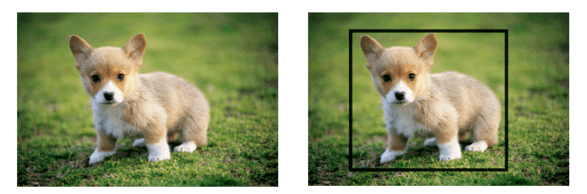
\includegraphics[width=\textwidth]{clas_loc}
		\label{fig:clas}
	\end{figure}
	
	Many research groups have been very generous in releasing their 
	models to the open-source community. Some of the most well-known models, such as 
	AlexNet, VGGNet, Inception, ResNet, Xception \citep{Krizhevsky_alexnet, Simonyan_vgg, 
	Szegedy_inception, He_resnet, Chollet_xception} won in the \acronym{ilsvrc}. 
	And others, like SqueezeNet, MobileNet \citep{Iandola_squeezenet, Howard_mobilenet} 
	etc participated in it.
	\par
	\citet{Krizhevsky_alexnet} 
	are widely regarded to have done one of the most influential publications in the field. 
	Because of AlexNet, 2012 marked the first year where a convolutional network was used to 
	achieve a top 5 test error rate of 15.3\%. The next best entry achieved an error 
	of 26.2\%, which was an astounding improvement that pretty much shocked the computer 
	vision community. \term{Top 5 error} is called the rate at which, given an image, 
	the model does not output the correct label with its top 5 predictions. AlexNet 
	really illustrated the benefits of convolutional networks and backed them up with 
	record breaking performance in the \acronym{ilsvrc}. Since then the use of convolutional 
	neural networks for classification has dominated the field.
	\par
	\citet{Simonyan_vgg} reinforced the notion that \defn{convolutional neural networks 
	have to have a deep network of layers in order for this hierarchical representation 
	of visual data to work}. VGGNet is characterized by its simplicity, using very small 
	(3$\times$3) convolutional filters, instead of AlexNet’s (11$\times$11), stacked on 
	top of each other in increasing depth from 16 to 19 layers. It was best utilized with 
	its 7.3\% error rate. But it is painfully slow to train.
	\par
	The original incarnation of the Inception architecture used in \citet{Szegedy_inception} 
	submission to \acronym{ilsvrc} 2014 is called GoogLeNet. It is a 22 layer convolutional 
	neural network. It actually uses 12 times fewer parameters than the winning architecture 
	AlexNet, from two years ago. It is also significantly more accurate, with a top 
	5 error rate of 6.7\%. Inception was one of the first models that introduced the 
	idea that convolutional layers did no always have to be stacked up sequentially, 
	but could perform many operations in parallel. Finally this new model places notable 
	consideration on memory and power usage.
	\par
	Depending on their skill and expertise, humans generally hover around a 5\%-10\% 
	error rate \citep{Deshpande}. But \citet{He_resnet} came up with the ResNet 
	architecture that has an incredible error rate of 3.6\%. Aside from the new record 
	in terms of error rate, ResNet is well-known due to its extreme depth of up to 152 
	layers. This is 8 times deeper than VGGNet. ResNet is also a great innovation for 
	the idea of residual learning.
	\\
	
	\begin{figure}[h!]
		\caption{Object Detection locates and identifies multiple objects and all their 
		instances (\textcolor{red}{cat}, \textcolor{blue}{dog}, \textcolor{green}{duck}) 
		within the image.}
		\centering
		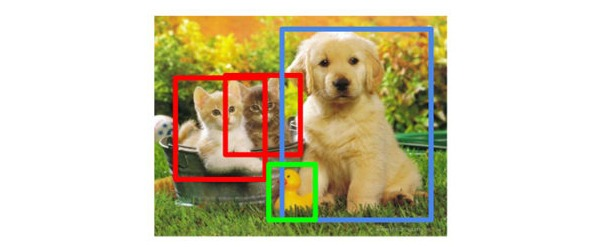
\includegraphics[width=\textwidth]{detect}
		\label{fig:det}
	\end{figure}
	
	Image classification is a lightweight form of object detection. The difference between 
	them is that in classification algorithms the goal is to label an image with a category 
	of the object it belongs (or at least the most likely predictions). While in detection 
	algorithms the aim is to draw a bounding box around the object of interest to locate it 
	within the image, as shown in Figure~\ref{fig:det}. Also, it is not necessary to draw 
	just one bounding box in the object detection case. There could be many bounding boxes 
	representing different objects of interest within the image, the number of which is 
	known a priori.
	\par
	A naive approach to do that would be to take different regions of interest from the 
	image by sliding windows from left and right, and from up to down. And then use a 
	convolutional network to classify the presence of the object within the chosen region. 
	The problem with this approach is that the objects of interest might have different 
	spatial locations and aspect ratios. Hence, the number of regions would be huge leading 
	to computationally blow up. Therefore, algorithms like \acronym{ssd}, \acronym{yolo} 
	and \acronym{r-cnn} \citep{Girshick, Redmon, Liu} have been developed to find these 
	occurrences in the fastest way possible. The aforementioned models are also released 
	to the open-source community.
	\par
	To bypass the problem of selecting a huge number of regions, \citet{Girshick} proposed 
	a method called \term{\acronym{r-cnn}: Regions with \acronym{cnn} features}, one of the 
	most impactful advancements in computer vision \citep{Deshpande}. The process can be 
	split into two general components, the region proposal step and the classification step. 
	For the former step, a selective search \citep{Uijlings} is used to extract just 2000 
	regions from the image that have the highest probability of containing an object. The 
	authors called them region proposals. These 2000 candidate region proposals are warped 
	into a square and fed into a trained convolutional network (VGGNet or AlexNet in this case) 
	that acts as a feature extractor. In the latter step, the extracted features are used to 
	classify the presence of the object within that candidate region proposal and to refine 
	the boundary box with the most accurate coordinates. The main disadvantage here is that 
	it still takes a huge amount of time to train the network as there 2000 region proposals 
	per image to classify. Also, the selective search algorithm is a fixed algorithm. Therefore, 
	no learning is happening at that stage, something that could lead to generating bad 
	candidate region proposals. That is why \term{Fast \acronym{r-cnn}} and 
	\term{Faster \acronym{r-cnn}} followed up.
	\par
	But, as an alternative, is a separate region proposal step needed? Can both boundary 
	boxes and classes directly from feature maps in one step? \citet{Redmon} use a single 
	convolutional network to predict the bounding boxes and the class probabilities for 
	these boxes. The use a \term{single shot object detection} algorithm called 
	\term{\acronym{yolo}: You Only Look Once}, that is much different from the 
	\term{region based detection} algorithm mentioned above. \acronym{yolo} divides every 
	image into a S $\times$ S grid and every grid predicts N bounding boxes and class 
	probability for them. The bounding boxes having the class probability above a threshold 
	value are selected and used to locate the object within the image. Note that at runtime, 
	the image runs on the convolutional network only once. Hence, \acronym{yolo} is super 
	fast and can be run real time. It sees the complete image at once as opposed to looking 
	at generated region proposals. However, a limitation for \acronym{yolo} is that it only 
	predicts one type of class in each grid. Hence, it struggles with very small objects.
	\par
	Yet another algorithm was developed by \citet{Liu}. \term{\acronym{ssd}: Single Shot 
	Detector} differs from others single shot detectors due to the usage of multiple layers 
	that provide a finer accuracy on objects with different scales. \acronym{ssd} runs a 
	trained convolutional network (for example VGGNet model) on input image only once and 
	calculates a feature map. Then it runs a 3 $\times$ 3 sized convolutional filter on 
	this feature map to foresee the bounding boxes and classification probability. It 
	attains a good balance between speed and accuracy.
	\\
	
	\begin{figure}[h!]
		\caption{Semantic Segmentation makes a prediction at every pixel within an image. 
		That means there is a label for each pixel, instead of object (\textcolor{green}{grass}, \textcolor{orange}{cat}, \textcolor{purple}{tree}, \textcolor{blue}{sky}). Original 
		image (left), output of the semantic segmentation (right).}
		\centering
		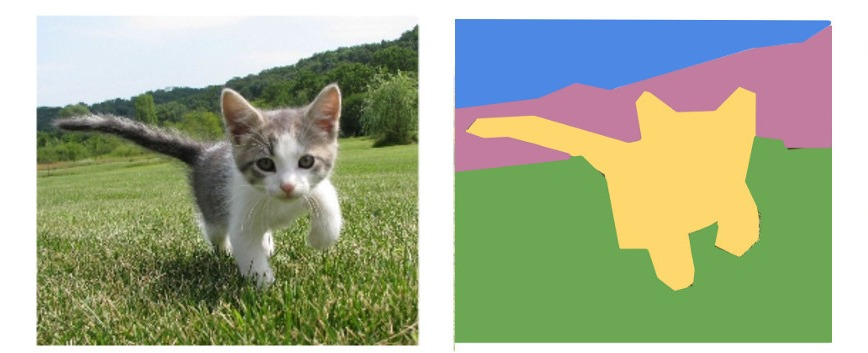
\includegraphics[width=\textwidth]{segm}
		\label{fig:segm}
	\end{figure}
	
	Nowadays, \term{semantic segmentation} is one of the key problems in the field of 
	computer vision \citep{Le}. Looking at the big picture, semantic segmentation is one 
	of the high-level task that paves the way towards complete scene understanding. 
	Although humans perform scene segmentation with apparent ease, automatic scene 
	segmentation is a very challenging problem \citep{Wang}. Segmentation refers to the 
	process of mapping each pixel in an image to an object class. Each object class has 
	to be segmented separately. For example see Figure~\ref{fig:segm}. As one can imagine, 
	this is a much more complex problem as compared to the classification or even detection 
	problem. The importance of scene understanding as a core computer vision problem is 
	highlighted by the fact that an increasing number of applications nourish from inferring 
	knowledge from imagery. Some of those applications include self-driving vehicles, 
	human-computer interaction, virtual reality etc. With the popularity of deep learning 
	in recent years, many semantic segmentation problems are being tackled using deep 
	architectures, most often convolutional neural networks, which surpass other 
	approaches by a large margin in terms of accuracy and efficiency.
	\par
	Probably the most well known models concentrating on scene segmentation are 
	\term{Fully Convolutional Neural Networks (\acronym{fcn}s)} \citep{Long}. The original 
	fully convolutional network is trained for pixel-wise prediction, without extracting 
	the region proposals. The authors adapt contemporary classification networks (AlexNet,
	VGGNet and GoogLeNet) into fully convolutional networks and transfer their learned 
	representations by \term{fine-tuning} to the segmentation task. Fine-tuning is a 
	process in which a network model that has already been trained for a given task, is 
	modified in order to perform another similar task. The main idea of fully convolutional 
	networks is to make classical convolutional networks take as input arbitrary-sized 
	images. Contrary to them, fully convolutional networks only have convolutional and 
	pooling layers which give them the ability to make predictions on arbitrary-sized inputs. 
	\term{Pooling layers} are in charge of reducing the number of parameters when the images 
	are too large. The results of the original fully convolutional networks are shown in 
	Figure~\ref{fig:fcn}.
	
	\begin{figure}[h!]
		\caption{Fully Convolutional Neural Networks: Original image (left), predicted label 
		map (right). Notice the predictions are only for the foreground, the entire background 
		in the left image appears black on the right.}
		\centering
		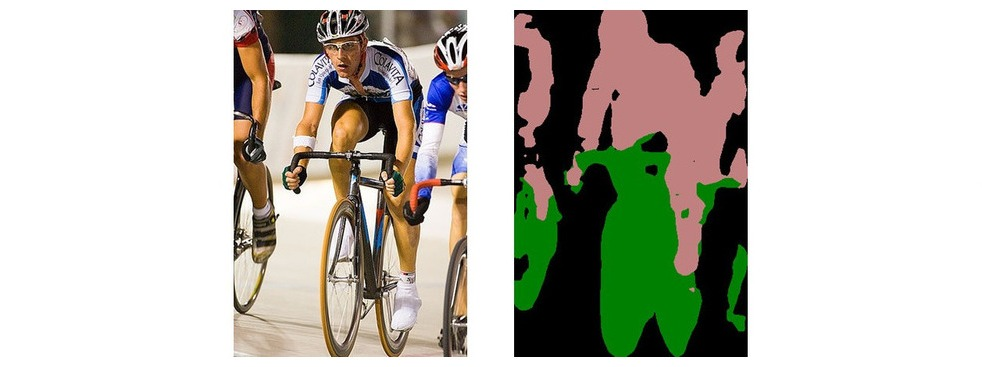
\includegraphics[width=\textwidth]{fcn}
		\label{fig:fcn}
	\end{figure}
	
	
	But what is the strategy for deciding where to go next? Is there a specific goal 
	for the robot to reach? Should it find the best trajectory? Explore the 
	environment? A discussion of this topic is made in the following section.
	\\
	
	\section{Navigation strategies}
	\label{sec:bg:goals}
	
	A natural thing would be to let the robot learn about the traversability 
	of the environment, while another perspective would be to concentrate on more 
	preservative situations, such as go or no-go \citep{Hirose}. Even though the 
	former method allows the robot to autonomously learn a model of the environment,
	encourages exploration and consequently improves the learning and generalization 
	performance \citep{Zhelo}, the trial and error part of it involves a high risk to 
	damage the robot. The latter, on the other hand, has as main priority to prevent 
	robots from colliding with objects, injuring people, getting stuck in constrained 
	spaces, or falling over an edge. 
	\par
	A third approach would be to let the autonomous vehicle navigate from a defined 
	start point to a fixed goal	point \citep{Shneier, Zhelo}. That way the robot has 
	to build a model of the world around it and plan a path from the start to the 
	goal. A way to do that is to enable the robot to learn which regions to avoid 
	and which to seek out, in early runs, so that in later runs it can determine the 
	most efficient path \citep{Shneier}. In cases where there is no the knowledge of 
	the map of the robot's current environment, the designated goal location can be 
	acquired via cheap localization solutions, such as visible light localization, 
	Wi-Fi signal localization or \acronym{gps} \citep{Zhelo}.
	\\
	
	Generally, \term{intrinsic motivations} are related to curiosity, exploration, 
	the interest for novel objects and surprising events and the interest in 
	learning new behaviors. They come in contrast to \term{extrinsic motivations} 
	which are to obtain biologically relevant resources to avoid damage and vouch 
	survival.
	\par
	In robotics, extrinsic motivations can be related to the accomplishment of the 
	user tasks assigned to the robot. In contrast, intrinsic motivations drive 
	behavior and actions to gain knowledge: e.g., to explore the world, to learn to 
	predict novel or surprising stimuli, to acquire a higher competence to change 
	the environment with action.
	\\
	
	\todo[size={{\scriptsize}}]{Something that is missing from the strategies deciding where to go next}
	In our knowledge, most approaches concentrate on robot navigation in order to 
	make sure they do not collide with other objects and they follow a route to 
	reach a specific goal. There is not much work done on curiosity-driven 
	exploration, where there is no explicit goal, but the abstract need for the 
	robot to learn a new environment. The traversability estimation is most commonly 
	performed in order for the robot to move safely rather than explore the 
	environment and learn which areas are traversable and which are not.
	\\
		
	\section{Conclusions}
	\label{sec:bg:concl}
	
	Intrinsic motivations fully entered the field of machine learning and robotics 
	only recently. That is despite some early pioneering computational explorations, 
	and although they were investigated by psychologists for a long time. Intrinsic 
	motivations are very important for autonomous robotics. They allow the acquisition 
	of knowledge and skills, in the absence of tasks directly established by the robot 
	users, e.g. to learn to manipulate different objects without being instructed to 
	do so. Also they are task-independent. That means they can drive the robotic system 
	to acquire skills re-usable to accomplish many possible tasks in a certain class 
	of environments.
	\\
	
	It has become clear to researchers in robotics and adaptive behavior that 
	current approaches are yielding systems with limited autonomy and capacity for 
	self-improvement. To learn autonomously and in a cumulative fashion is one of 
	the hallmarks of intelligence, so that is what we want to achieve in the current 
	thesis. The traversability estimation can become a goal of action based on 
	intrinsic motivations.
	\\
	
	We explored many ways for a robot to be able to decide for itself the 
	traversability of the terrain around it and plan paths to avoid any obstacles. 
	We also investigated ways to improve the robot's traversability estimation 
	method in everyday practical situations. So, this thesis will be focused on the 
	one thing that is missing; intrinsically motivated learning. It will mainly 
	concentrate on how to explore the environment around the robotic platform and 
	improve its knowledge of traversability.
	\\\\
	
	Enough of background, let’s now see how our autonomous mobile robot takes input 
	from its environment and handles the newly acquired knowledge to improve its 
	traversability estimation method.
	\\
	
	
	\chapter{Core Foreground}
	\label{sec:fg}
	
	\section{A few words}
	\label{sec:fg:intro}
	
	Our goal is for the robot to be able to autonomously navigate in natural environments. 
	To do so, we could use a pre-trained neural network in order to be able to distinguish 
	traversable from non-traversable terrain.
	\par
	For the purposes of this thesis we will basically deal with pre-trained models. By
	borrowing a little story from \citet{Gupta} we are going to explain why. Imagine two 
	people, Mr. Potato and Mr. Athlete. They sign up for soccer training at the same time. 
	Neither of them has ever played soccer and the skills like dribbling, passing, 
	kicking etc. are new to both of them. Mr. Potato does not move much but Mr. Athlete 
	does. That is the core difference between the two even before the training has even 
	started. As you can imagine, the skills Mr. Athlete has developed as an athlete 
	(e.g. stamina, speed and even sporting instincts) are going to be very useful for 
	learning soccer even though Mr. Athlete has never trained for soccer. Mr. Athlete 
	benefits from his pre-training. Mr. Potato on the other hand will have to develop all 
	these skills from scratch, something that will cost him much more energy and time.
	\\
	
	\section{Initial attempts / efforts}
	\label{sec:fg:at}
	
	The first attempt was to use one of the most-well known models from \acronym{ilsvrc}. 
	With a little help from the code of \citet{Rosebrocke} we experimented on 
	pre-trained VGGNet, ResNet, Inception and Xception. We fed them images and, 
	as expected, they returned classification predictions about them. With the 
	contribution of ImageNet a list of human-readable labels and the probability 
	associated with them was printed.
	\par
	Images containing just one object (e.g. soccer ball, couch) led to predictions 
	that were satisfactory in their entirety. But being fed with images containing 
	multiple objects (e.g. book and glasses) the networks got confused. They gave 
	some decent predictions (like envelope or book jacket, in the previous example) 
	but also some that were a little bit off (like lighter or birdhouse), within 
	their top-5 list.
	\par
	Images that contain vegetation, which are of particular interest to us in this work, 
	were the worst case scenario. For example, the networks above, after being fed with 
	an image of a tree, gave as most likely predictions kinds of seeds like lemons. This 
	probably happened because the networks concentrated on the one part of the whole image 
	that was most recognizable by them. Finding out what the predictions with smaller 
	probabilities were, did not help. As the networks kept predicting, they got desperate 
	and started giving all sorts of provisions. 
	\par
	Even though these networks are proven to be great on object classification, when 
	it comes to scene recognition there is no trivial way to make them work correctly.
	\par
	Similarly, models specialized in object detection like \acronym{ssd} or \acronym{yolo}, 
	do not seem to be able to generalize on scene segmentation issues. As dictated by their 
	name, they detect all objects within an image, but ignore the rest of the scene.
	\\
	
	Many papers have been published regarding robot navigation approaches that use 
	already existing deep neural networks, or modify them in order to meet their needs.
	Unfortunately some of these researchers had not made their code publicly available, 
	in order for us to rely on part of their work and extend it with our own ideas. And 
	while others kindly released their code online, their networks were not trained 
	compatible to the needs of this thesis.
	\par
	Some papers considering traversability estimation concentrate on go or no-go situations, 
	\citep{HiroseGonet, HiroseVunet}. They use generative adversarial networks and train 
	them to estimate whether the space seen through the given image is traversable or not. 
	They are trained in indoor environments, which means that we would have to train them 
	from scratch to work in natural outdoor environments.
	\par
	Likewise, \citet{Tai} further extended the concept of deep neural networks to not only 
	perception but also decision-making. Basically, they used a structure that fuses several 
	convolutional neural network layers with decision-making process, in order to explore 
	an unknown environment. According to the writers, in traditional computer vision 
	applications each label of the output represents either an object or scene categories. 
	The outputs of their model are control commands that show the platform which route to 
	follow.
	\par
	Other researchers use neural networks to classify the area in front of the robot 
	according to traversability and level of confidence \citep{Sermanet, Hadsell}. These 
	neural networks assign class labels to parts of the input image. Classes which show 
	that \defn{only ground or only obstacle is seen in window}, are of high confidence. 
	While the rest inspire lower confidence. These classes are separated to 
	\defn{ground and obstacle may be seen}, \defn{obstacle is seen but does not fill window}, 
	\defn{location where an obstacle meets the ground}.
	\par
	Some approaches identify only a few class labels to classify the whole image 
	\citep{Holder, Bosch, Farabet}. While others have as their main goal to find and follow 
	a path \citep{Yang, Orsic}. The first category usually includes class labels that can 
	be used in outdoor environments, as their title declares (such as sky, road, tree, grass, 
	building). The second one, while also being able to recognize such class labels, 
	identifies them as obstacles.
	\\
	
	So, the aim is on total scene segmentation rather than single or even multiple object 
	categorization. Semantically meaningful image understanding is a relatively recent topic 
	in computer vision. That explains why, compared to recognition, far fewer papers address 
	scene segmentation in neural networks \cite{Wang}. A general semantic segmentation 
	architecture can be broadly thought of as an \term{encoder network} followed by a 
	\term{decoder network} \citep{Le}. The encoder is usually a pre-trained classification 
	network like VGGNet or ResNet that outputs a feature map. The task of the decoder is 
	to semantically project the lower resolution features learned by the encoder, onto the 
	higher resolution (pixel space) to get the best closest match to the original input.
	\par
	Following the instructions of \citet{Le} we attempted to implement the most popular 
	architecture for semantic segmentation, fully convolutional networks. We had in mind 
	that the encoder, VGGNet in this case, would be pre-trained, but we would have to 
	train the decoder from the beginning. But fully convolutional networks, at least 
	on the cases we saw them used, do semantic segmentation only on foreground and ignore 
	the background (Figure~\ref{fig:fcn}). In order for us to be able to decide terrain 
	traversability, whole scene segmentation is necessary.
	\\
	
	ADE20K dataset
	\\


	
	
	
	
	
	
	
	
	Failed trials:
	
	Vision-Based Real-Time Traversable Region Detection for Mobile Robot in the Outdoors -> no available code
	Fast Road Scene Segmentation using Deep Learning and Scene-based Models -> road, obstacles, sky
	Pixel-wise Segmentation of Street with Neural Networks -> just street
	
DeepLab (\url{https://github.com/tensorflow/models/tree/master/research/deeplab} 
\& \url{https://gluon-cv.mxnet.io/build/examples_segmentation/index.html} -> getting .param files)

and datasets:
PLVP dataset -> pedestrian lane
KITTI dataset -> road and lane detection, asphalt roads
Stanford background dataset -> grass and tree as classes
ADE20K -> whole image segmentation
COCO, PASCAL VOC -> semantic for foreground only
	
	thesis (no code available):
	Road Detection and Recognition from Monocular Images Using Neural Networks -> image has road or not,
	Autonomous Terrain Classification Through Unsupervised Learning -> neural network trained on colour, depth and infrared data,
	Semantic Segmentation for Terrain Roughness Estimation Using Data Autolabeled with a Custom Roughness Metric -> roughness of each path
	\\\\
	
	
	
	
	
	\section{Our approach}
	\label{sec:fg:app}
	
	
	\todo[size={{\tiny}}]{In: Arbib M.A. (ed.), The Handbook of Brain Theory and Neural Networks, 2nd Ed., MIT Press, Cambridge MA, pp. 1215-1219, 2003.}
		
	\todo[size={{\scriptsize}}]{Datasets? COCO, Pascal VOC, ADE20K, PLVP, KITTI, Stanford background?}

	\todo[size={{\scriptsize}}]{ADE20K (dataset that has densely annotated images) scene parsing \& semantic segmentation -> matlab \& PyTorch}
	
	\todo[size={{\scriptsize}}]{DeepLab using ADE20K (what happened when used other dataset?)}
	
	
	\todo[size={{\scriptsize}}]{Semantic Segmentation, Urban Navigation, and Research Directions (Qasim Nadeem) -> not in Google Scholar -> ???}
	
	
	
	
	
	\chapter{Experimental Validation and Comparison}
	\label{sec:exp}
	
	\section{Evaluation setup}
	\label{sec:exp:eval}
	
	\section{Results}
	\label{sec:exp:res}
	
	\section{Discussion}
	\label{sec:exp:dis}
	
	
	\chapter{Conclusions and Future Work}
	\label{sec:concl}
	
	
	\appendix
	\chapter{Prototype / Reference Implementations}
	\label{app:impl}
	
	Many writers published their code open-source so that other researchers may 
	use their work. Here we give some \acronym{url}s and comments about the work 
	mentioned above in Section~\ref{sec:bg:trav}, Section~\ref{sec:bg:data} and 
	Chapter~\ref{sec:fg}. Some of them were actually used as our experimental basis.
	\\
	
	\begin{table}[h]
		\centering	
		\begin{center}
\resizebox{\textwidth}{!}{%
\begin{tabular}{cc}
	Authors & \acronym{url}\\ 
	\hline\hline
	\citet{Droeschel} & \url{https://github.com/AIS-Bonn/mrs_laser_map}\\
	\citet{HiroseGonet} & \url{https://github.com/NHirose/GONET}\\
	\citet{Goodfellow} & \url{http://www.github.com/goodfeli/adversarial}\\
	\citet{Krizhevsky_alexnet} & \url{https://github.com/Abhisek-/AlexNet}\\
	\citet{Simonyan_vgg} & \url{http://www.robots.ox.ac.uk/~vgg/research/very_deep/}\\
	\citet{Szegedy_inception} & \url{https://github.com/google/inception}\\
	\citet{Chollet_xception} & \url{https://github.com/kwotsin/TensorFlow-Xception}\\
	\citet{He_resnet} & \url{https://github.com/KaimingHe/deep-residual-networks}\\
	\citet{Iandola_squeezenet} & \url{https://github.com/DeepScale/SqueezeNet}\\
	\citet{Howard_mobilenet} & \url{https://github.com/Zehaos/MobileNet}\\
	\citet{Tai} & \url{https://github.com/libcnn/libcnn}\\
	\citet{Girshick} & \url{https://github.com/rbgirshick/rcnn}\\
\end{tabular}
}
\end{center}


\url{http://groups.csail.mit.edu/vision/datasets/ADE20K/}\\
\url{https://github.com/CSAILVision/semantic-segmentation-pytorch}	
	\end{table}
	
	
	\chapter{Basic information on Convolutional Neural Networks}
	\label{app:conv}
	
	Based mainly on \citet{Deshpande_guide} beginner's guide, we give a brief 
	description on convolutional neural networks.
	\\
	
	When a computer takes an image as input, it sees an array of pixel values. This 
	array is sized depending on the resolution and size of the image. Let's say we 
	have a color image in \acronym{jpg} form and its size is 32 $\times$ 32. The 
	representative array will be 32 $\times$ 32 $\times$ 3 (the 3 refers to \acronym{rgb} 
	values). Each of these numbers is given a value from 0 to 255 which describes the 
	pixel intensity at that point. These numbers, while meaningless to us when we 
	perform image classification, are the only inputs available to the computer. The 
	idea of neural networks is that we give the computer this array of numbers and 
	it outputs numbers that describe the probability of the image being a certain 
	class (e.g. 80\% for cat, 15\% for dog, 5\% for bird etc).
	\\
	
	So what we want the computer to do is to be able to differentiate between the 
	images it is given and figure out the unique features that make a dog a dog or 
	that make a cat a cat. This is what human minds do subconsciously as well. Roughly,
	we can classify a dog in a picture if it has identifiable features such as paws or 
	snout or four legs. In a similar way, the computer is able perform image 
	classification by looking for low level features such as edges and curves, and 
	then building up to more abstract concepts like paws and beaks, through a series 
	of convolutional layers. This is a general overview of what a convolutional neural 
	network does.
	\\
	
	The first layer in a convolutional neural network is always a \term{convolutional 
	layer}. The best way to explain a convolutional layer is to imagine a flashlight 
	that is shining over the top left of the image. Let’s say that the light this 
	flashlight shines covers a 5 $\times$ 5 area. And now, let’s imagine this flashlight 
	sliding across all the areas of the input image. In machine learning terms, this 
	flashlight is called a \term{filter} (also referred to as a \term{neuron} or a 
	\term{kernel}) and the region that it is shining over is called \term{receptive 
	field}. This filter is also an array of numbers called \term{weights} or 
	\term{parameters}. A very important note is that the depth of this filter has to 
	be the same as the depth of the input (in order for the math to work out), so the 
	dimensions of this filter is 5 $\times$ 5 $\times$ 3. 
	\par
	As the filter is sliding, or \term{convolving}, around the input image, it is 
	multiplying the values in the filter with the original pixel values of the image 
	(aka computing \term{element wise multiplications}). Mathematically speaking, this 
	would be 75 multiplications in total for the first position the filter is in. Then 
	these multiplications are all summed up to a single number. The next step is to 
	move the filter to the right by one unit and repeat. This process is repeated for 
	every location on the input volume and produce a number.
	\par
	There are 784 different locations that a 5 $\times$ 5 filter can fit on a 
	32 $\times$ 32 input image. So after sliding the filter over all the locations, 
	the result is an 28 $\times$ 28 $\times$ 1 array of numbers, called an \term{activation 
	map} or \term{feature map}. Using more filters makes possible to preserve the spatial 
	dimensions. If there are two 5 $\times$ 5 $\times$ 3 filters used instead of one, 
	the output volume would be 28 $\times$ 28 $\times$ 2. The more filters, the greater 
	the depth of the activation map, and the more the information about the input image.
	\par
	Each of these filters can be thought of as \term{feature identifiers}, for features 
	like straight edges, curves, simple colors. For example, let's assume one filter 
	is a curve detector. If there is a shape in the input image that generally resembles 
	the curve that this filter is representing, then all of the multiplications summed 
	together will result in a large value. And if not, the value will be much lower. 
	This will happen if there is nothing in the image section that responds to the 
	curve detector filter. So the activation map will have large values in the areas 
	where is most likely to have curves, and low values on the least likely.
	\\
	
	Moving to the next layer, its input would be the output of the previous layer. 
	In this case the input of the second layer will be the activation maps that result 
	from the first layer. So the input is basically describing the locations in the 
	original image where certain low level features appear. Applying a set of filters 
	on top of that, as it passes through the second convolutional layer, the output 
	will be activations that represent higher level features. Types of these features 
	could be semicircles (i.e. combination of a curve and straight edge) or squares 
	(i.e. combination of several straight edges).
	\par
	As going through the network and through more convolutional layers, the activation 
	maps represent more and more complex features. By the end of the network, there 
	might be some filters that activate when there is handwriting in the image, when 
	they recognize green objects, etc. An interesting thing to note is that going deeper 
	into the network, the filters begin to have a larger receptive field. That means 
	they are able to consider information from a bigger region of the original input 
	volume.
	\\
	
	Finally, at the end of the network there is a \term{fully connected layer}. This 
	layer takes as input the output from the layer preceding it, and outputs a vector 
	with dimensions the number of classes that the program has to choose from. Each 
	value of the vector represents the probability of a certain class.	For example, 
	let's take a digit classification program. The output the a dimensional vector 
	such as [0 0.1 0.1 0.75 0 0 0 0 0 0.05], since there are ten digits. This represents 
	a 10\% probability that the original image is a 1, a 10\% that it is a 2, a 75\% 
	that it is a 3, and a 5\% that it is a 9. Basically, a fully connected layer take 
	the activation maps of the previous layer and determines which features most 
	correlate to a particular class.
	\\
	
	
	\renewcommand{\bibname}{References}
	\bibliography{ref}
	\bibliographystyle{unsrtnat}
\end{document}